\section{Introdu��o}

O prop�sito deste trabalho � o de permitir a utilizadores a execu��o de opera��es geom�tricas sobre
modelos tridimensionais.
As opera��es devem ser fornecidas ao utilizador de forma contextual, no pr�prio ambiente de visualiza��o,
fornecendo um conjunto de restri��es direccionais de modo a auxili�-lo a obter o efeito desejado.

A aplica��o de uma opera��o inicia-se com a selec��o atrav�s de um tra�o de uma face ou aresta a afectar,
o que despoleta o aparecimento de um menu contextual.
O utilizador escolhe ent�o a opera��o a aplicar, sendo esse mesmo tra�o interpretado para determina��o
dos par�metros da opera��o.

O sistema foi implementado como funcionalidade do prot�tipo multimodal ImmiView presente no laborat�rio Louren�o Fernandes
do IST Tagus Park \cite{leme}, permitindo a sua aplica��o em cen�rios com tablet PCs ou ecr�s de larga escala.

\begin{figure}[!ht]
	\centering
	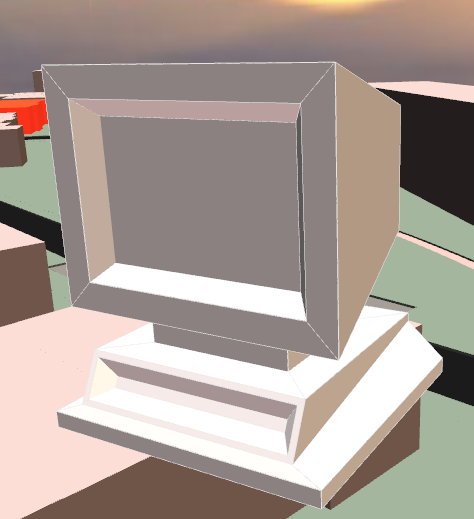
\includegraphics[width=0.4\linewidth]{ex-monitor.png}
	\vspace{-3mm}
	\caption{monitor modelado no sistema}
	\label{fig:example}
	\vspace{-3mm}
\end{figure}